\scanpage{265}
d'où la conclusion

Le cas qui nous intéresse est
\[
N'_0=0\leq N,\quad C=\operatorname{Mod}(k),
\]
\(i(M)=M\otimes_k S,\) et si on sait que
\[
M\otimes_k S\subset\operatorname{Imess}\varphi_{0N}\qquad\forall M\in\operatorname{Mod}(k)
\]
i.e.
\[
M\otimes_k S\simeq\varphi_{0N}\tau_N(M\otimes_k S)
\bigl(=R^0\varphi_{0N}(\unsure{\tau_N M\otimes_k S})\bigr)
\]
\[
\deleted{\unsure{\Vert}\quad\operatorname{Hom}((\tau_{N-i}S)[-i],M\otimes_{\unsure{k}})}
\]
alors on a
\[
R^n\varphi_{0N}(\tau_N(M\otimes_k S))=0\quad\text{si }n>0
\]
i.e.
\[
\boxed{\operatorname{Ext}^n_{\mathcal M}((\tau_{N-i}S)[-i],M\otimes_k S)=0\quad\text{si }n>0,\ i\geq0}
\]
\figure{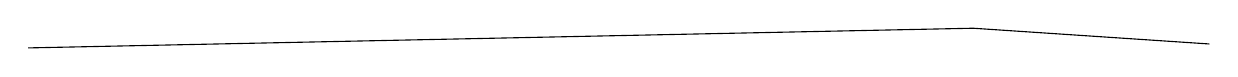
\begin{tikzpicture}\draw (0,0)--(12,.25)--(15,.05);\end{tikzpicture}}
\[
\operatorname{Hom}_{\mathcal M}(M,\varphi_\infty\tau_\infty P)\simeq\ldots
\underset{\text{si }M\text{ de prés. finie}}{\simeq}
\varinjlim_N\operatorname{Hom}_{\mathcal M}^{\deleted{\unsure{*}}}(\tau_{N\deleted{\unsure{-i}}}M,\deleted{\unsure{\tau}}P)
\]
Si de plus \(M\) projectif
\[
\operatorname{Hom}(M,R^*\varphi_\infty(\tau_\infty P))\simeq
\varinjlim_N R\operatorname{Hom}_{\mathcal M}((\tau_{N\deleted{\unsure{-i}}}M)\deleted{\unsure{[-i]}},-)
\]
en particulier
\[
\operatorname{Hom}(M,R^n\varphi_\infty P)\simeq
\varinjlim_N\operatorname{Ext}_{\mathcal M}^n((\tau_{N-i}M)[-i],P)
\]
p.ex. si \(M=S[i],\) on trouve
\[
\deleted{R^*}(\varphi_\infty\tau_\infty P)_i=
\varinjlim_N\operatorname{Hom}^i(\tau_{N-i}S,P)
\]
\[
(R^*\varphi_\infty(\tau_\infty P))_{\unsure{i|0}}\simeq
\varinjlim_N R^*\operatorname{Hom}^i(\tau_{N-i}(S),P)
\]
\[
\deleted{\unsure{R\operatorname{Hom}^i}}
(R^n\varphi_\infty(\tau_\infty P))_i\simeq
\varinjlim_N\operatorname{Ext}_{\mathcal M}^n(\tau_{N-i}(S)[-i],P).
\]
\margin{264}
